\documentclass[twoside,11pt]{article}

% Any additional packages needed should be included after jmlr2e.
% Note that jmlr2e.sty includes epsfig, amssymb, natbib and graphicx,
% and defines many common macros, such as 'proof' and 'example'.
%
% It also sets the bibliographystyle to plainnat; for more information on
% natbib citation styles, see the natbib documentation, a copy of which
% is archived at http://www.jmlr.org/format/natbib.pdf

\usepackage{./jmlr2e}
\usepackage{amsmath}
\usepackage{subcaption}

% Definitions of handy macros can go here

\newcommand{\dataset}{{\cal D}}
\newcommand{\fracpartial}[2]{\frac{\partial #1}{\partial  #2}}

% Heading arguments are {volume}{year}{pages}{submitted}{published}{author-full-names}

\jmlrheading{1}{2020}{1-48}{4/00}{10/00}{Seth Bassetti, Ben Holmgren, and Wes Robbins}

% Short headings should be running head and authors last names

\ShortHeadings{Learning with Na{\"i}ve Bayes}{Bassetti, Holmgren, and Robbins}
\firstpageno{1}

\begin{document}

\title{Learning with Na{\"i}ve Bayes}

\author{\name Seth Bassetti \email seth.bassetti@student.montana.edu \\
       \addr School of Computing\\
       Montana State University\\
       Bozeman, MT, USA
	\AND
	\name Ben Holmgren \email benjamin.holmgren1@student.montana.edu \\
       \addr School of Computing\\
       Montana State University\\
       Bozeman, MT, USA
       \AND
       \name Wes Robbins \email wesley.robbins@student.montana.edu \\
       \addr School of Computing\\
       Montana State University\\
       Bozeman, MT, USA}
\editor{Seth Bassett, Ben Holmgren, and Wes Robbins}

\maketitle

\begin{abstract}%   <- trailing '%' for backward compatibility of .sty file
This paper describes our group's findings when using a Na{\"i}ve Bayesian
approach for learning on various sets of data. We provide our findings on
these data sets with and without noise in the data. More specifically, we show
how the model performs on each data set using a percent accuracy statistic
and two different loss functions. Prior to the project, we were expecting to find
that generally the model would perform best on data with more feature variables,
and also that the model would perform best on less noisy data. Though our
hypotheses were not fully confirmed to the degree of statistical significance
we had initially expected, we did find that these trends were present throughout
the project, with exceptions for specific cases.
\end{abstract}


\begin{keywords}
  Na{\"i}ve Bayes
\end{keywords}

\section{Problem Statement}
Utilizing five datasets- each from unique and differing settings, we implemented a
 Na{\"i}ve Bayesian learning model in an attempt to provide insights into the correlation 
 of features within each set of data. More rigorously, each data set came with explicit classifications,
  and we sought to train our model in order to then guess the classification of a given set of feature data
  in the absence of a provided classification. Each of the five datasets we use in the project have a variable 
  number of classes and either discrete or real valued attribute values. We then provided an analysis of each
  dataset with perturbations on its feature values. We hypothesized that in general, more attributes would mean
  a better performance of our model, since more attribute data could be interpreted as gaining greater specificity in
  pinpointing revealing characteristics of a class. We presumed that this enhanced performance would be statistically
  significant, in that at least 90 percent of trials would show greater reliability of learning on datasets with more attribute data 
  when compared to datasets with fewer attributes. In this context, the reliability of learning then was measurable by the percent with which the
  model correctly guessed a class given only feature data, and also via two loss functions of our choosing. Additionally, we
  hypothesized that any given dataset would perform more reliably 90 percent of the time when compared to its corresponding permuted
  data, under the same measurements for reliability as for the first hypothesis. 

\section{Methods}
In order to test our hypotheses, we ran our model on the five original given datasets and introduced noise into each dataset,
comparing the results that our learning model was able to attain when comparing the original data to data with perturbations.
Initially, the datasets we used to test our model included breast cancer screening data, data referring to different properties of
various kinds of glass, data on the properties of three different iris plant species, data referring to the properties of different 
kinds of soybeans, and the 1984 voting data of each congressman in the U.S. house of representatives on the sixteen key 
votes identified in the Congressional Quarterly Almanac. All of these data were real valued, with the exception of the data 
corresponding to the House of representatives, which was in the form of strings indicating a vote ``y" for yes and ``n" for no.
We converted these strings into real valued entries by assigning all yes votes to the value 1, and all no votes to the value 0.
We also needed to handle missing attribute values in our data, which were existent in two of our datasets. In the congressional
 voting dataset, missing values corresponded with a ``present" vote, or a refusal to take sides. For this, we assigned all missing 
 values 0, which corresponds to a ``no", since voting present most likely would indicate that the voter is against the proposal. 
 The breast cancer dataset also had missing values which actually corresponded to data which was unavailable. Because the dataset
  was already real valued on a range from 1 to 10, we decided to give all missing entries a value of 5 which corresponds to the midpoint
  of the range. We rationalized that in a medical setting, this should indicate that a queried cancerous bump shouldn't be negligently overlooked,
  but missing data also need not indicate severe cancer, so we decided that a middle value in this context was appropriate. 


For each of these data sets, noise was introduced by permuting
approximately 10\% of the feature data in any given set. More precisely, for each and every feature value, there was a randomized 10\%
chance that perturbation would occur. Perturbation was conducted by computing the midpoint of values for every feature, and then
``flipping" every selected data point over this midpoint by subtracting from the midpoint the distance between the midpoint and the data point
if the data point were initially larger than the midpoint, and otherwise adding to the midpoint the distance between the midpoint and the data
point if the point were initially smaller than the midpoint. 

Mathematically, letting $F_i$ be a feature in a dataset and $f _j\in F_i$ be an individual data point of $F_i$, a midpoint $m$ was computed by
$m = (max(f \in F_i) + min(f \in F_i))/2$, and our perturbations $f_j^*$ were then conducted by computing on the randomly selected $f_j$
composing approximately 10\% of $F_i$:

\[\begin{cases}
	f_j^*=m-(f_j-m) \text{ if $f_j > m$}\\
	f_j^*=m+(m-f_j) \text{ if $f_j < m$}
	\end{cases}\]

	
Having accomplished the perturbations, another step of preprocessing this data was discretizing real-valued data into categorical data. To do this, we used ``binning", 
which is the processing of dividing values into a number of bins in order to convert it into a finite number of categories. Initially, we
set the number of bins to 2 for every dataset before we would go back and fine tune hyperparameters once the algorithm was fully implemented.

After fully preprocessing our data, we were able to begin implementation of the Na{\"i}ve Bayesian algorithm. After doing so, we needed a metric to determine how well 
our algorithm performs on each dataset. For this task, we introduced two loss functions to measure performance, a 0/1 loss function, and a log based loss function. 
These loss functions provide an effective method of determining model performance when certain features of the model are changed. Explicitly, letting $c_i$ be the level 
of certainty with which a guess was made in our model for the $i$th line of test data, logarithmic loss for each data point was computed as follows:
\[\begin{cases}
	ln(c_i) \text{ if correct}\\
	ln(1-c_i) \text{ if incorrect}\\
\end{cases}\]
Letting the value $y_i$ be the value produced by the above equation for the $i$th line of test data, the logarithmic loss  for the entire test set $T$ is computed
as:
\begin{equation}
\frac{-1}{|T|}\sum_{t \in T}^{ } y_i
\end{equation}

%1-correct/total
The second loss function we introduced was the 0/1 loss function, which is the ratio of incorrect guesses to total guesses made on the testing data.
Again denoting the test set $T$, and letting the number of correct guesses made on the test set by the model be denoted $g_c$, the 0/1 loss is computed with the simple ratio:
\begin{equation}
	1 - \frac{g_c}{|T|}
\end{equation}

We chose both of the above loss functions with the motivation that both are relatively simple to compute, as all of the terms are directly attainable from the output of our algorithm, and
because they are metrics with importantly opposed qualities in the evaluation of a Bayesian model. Perhaps the most famous and immediately logical evaluation of loss is 0/1 loss, 
which is a measurement of the ratio of incorrect guesses made in a test set. Importantly, this is indicative of the accuracy of our model, but is not particularly informative of overfitting.
Logarithmic loss however is helpful when evaluating the performance of a model while also keeping in mind the potential of overfitting. By incorporating punishments for having a high degree
of certainty in an incorrect decision, logarithmic loss is useful in capturing the performance of a model with greater depth than simply counting the number of correct solutions- 
which in turn provides a weariness for overfitting.
Both metrics are important to have an effective model, so both loss functions were chosen in the evaluation of our model on various data.

Once our algorithm and loss functions had been fully implemented, we began tuning hyperparameters to optimize model performance. Ten fold cross validation proved to be a useful method of training and 
testing our data. This involved dividing the dataset into ten groups, with nine being used for training and one being used for testing, and rotating so that every group is eventually used for testing. The 
hyperparameter we were most interested in was the number of bins we used to discretize the real valued datasets. 
Using cross-validation, we determined that 4 bins offered the best performance for our model, and thus divided the real values into 4 bins to discretize it for features
with more than four independent values assigned to any given entry. This was due in part to our findings that the performance
of our model didn't seem to be altered once the bin size was increased above 4, and also due to some limitations in our implementation. Creating more bins seems to bog down
our model, and introduces a host of potential problem areas in our implementation that don't seem to be worth minimal performance improvements in the best case, and 
in practice no real noticeable difference. However, improving our ability to fine tune binning is a clear area for future work for subsequent implementations. Yet, for this
project, altering the number of bins seemed by observation to be around optimal with 4 bins for every feature in each dataset excluding the congressional voting data, 
which for practical purposes was also convenient in that it limited the number of areas where potential vulnerabilities could arise within our implementation.

\section{Results}

When running our learning algorithm on each of the datasets, we were able to quickly make observations as to which data our model was able to learn most effectively, and which sets of data
our model had a more difficult time with. Using our chosen loss functions described above, we could notice that the datasets that our model was able to learn best were noticeably the house
voting dataset and the breast cancer dataset, and their corresponding perturbations. The Iris data and glass data retained relatively low log loss values, but were more dispersed with respect 
to 0/1 loss. The soybean data was the worst performing dataset for our model under our chosen metrics with relatively scattered log loss and 0/1 loss values. To present the performance of our
model on each dataset under our chosen loss functions, we provide our results in the form of scatterplots whose y-axis is occupied by log loss values, and whose x-axis is occupied by 0/1 loss values.
In doing so, we've provided the visualization that high performing datasets under our metrics will appear clustered in the bottom left corner of each scatterplot.

Our experiment was conducted with 30 trials for each dataset using 10-fold cross validation for each trial, to provide the data presented in figures \ref{fig:good} and \ref{fig:ugly}. 
The mean log loss and 0/1 loss values for each dataset after 30 trials can be found in the following tables (where data with perturbation is denoted by *):

\begin{center}
 \begin{tabular}{|c c c c c|} 
 \hline
 Loss Function & Vote & Vote* & Cancer & Cancer*\\ [0.5ex] 
 \hline\hline
 0/1 Loss & 0.1041 & 0.1126 & 0.0348 & 0.0458\\ 
 \hline
 Log Loss & 0.5809 & 0.4401 & 0.1890 & 0.2116\\  
 \hline
\end{tabular}
\end{center}

\begin{center}
 \begin{tabular}{|c c c c c c c|} 
 \hline
 Loss Function & Glass & Glass* & Iris & Iris* & Soy & Soy*\\ [0.5ex] 
 \hline\hline
 0/1 Loss  & 0.2206 & 0.4297 & 0.2654 & 0.2092 & 0.4300 & 0.4350\\ 
 \hline
 Log Loss & 0.5194 & 0.7116 & 0.3633 & 0.3840 & 1.6919 & 1.706\\  
 \hline
\end{tabular}
\end{center}

\begin{figure}[h!]
  \centering  
   \begin{subfigure}[b]{0.6\linewidth}
    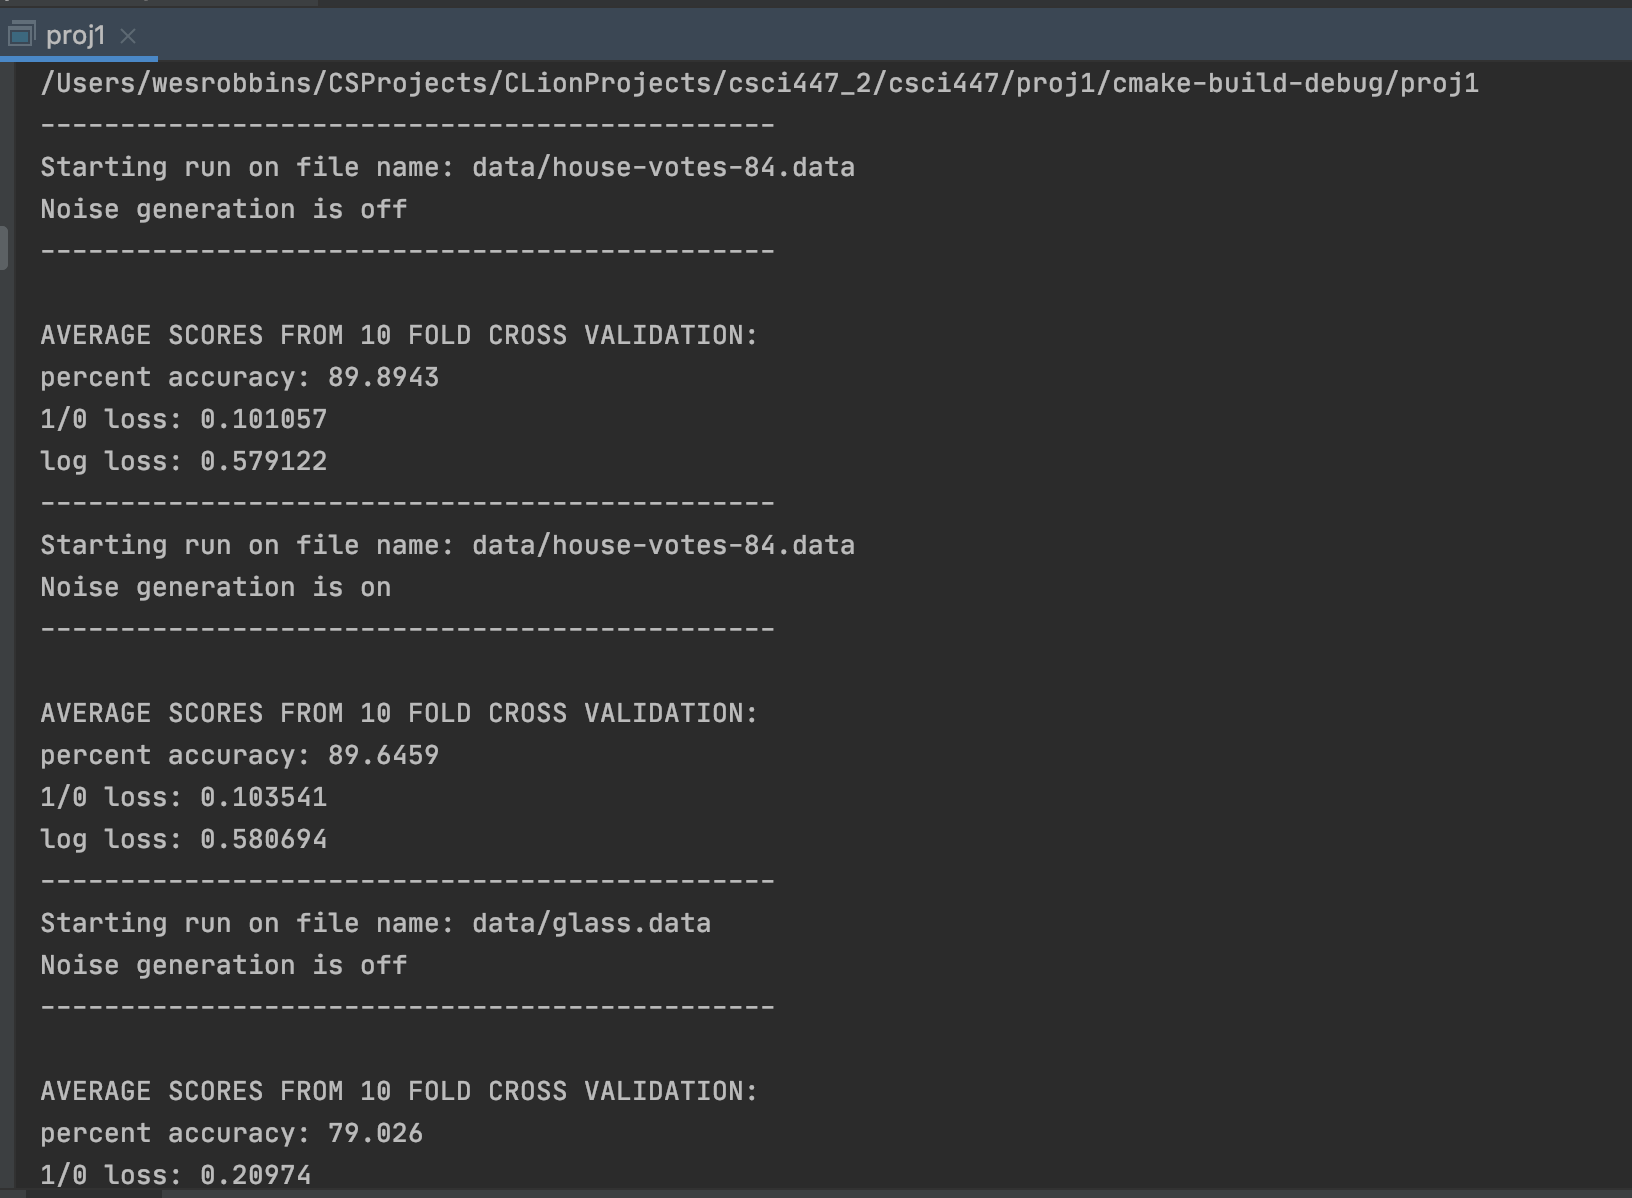
\includegraphics[width=\linewidth]{images/sample1.png}
  \end{subfigure}
  \begin{subfigure}[b]{0.6\linewidth}
    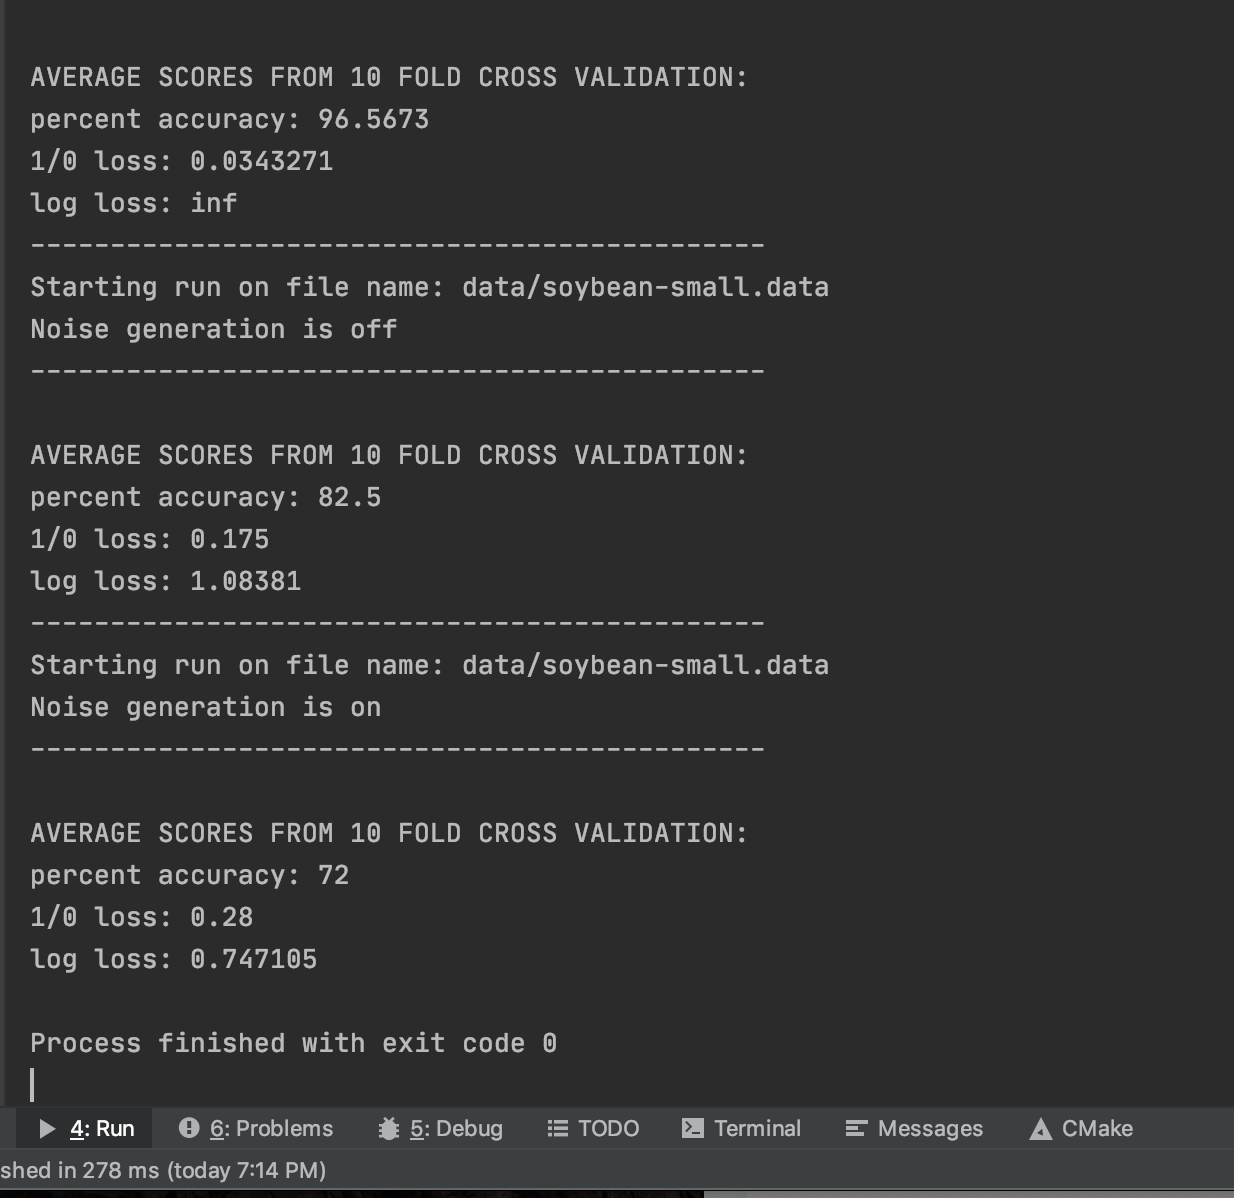
\includegraphics[width=\linewidth]{images/sample2.png}
  \end{subfigure}
  \caption{A sample run of our implementation of the algorithm on the unperturbed house voting data}
  \label{fig:good}
\end{figure}




\begin{figure}[h!]
  \centering
  \begin{subfigure}[b]{0.45\linewidth}
    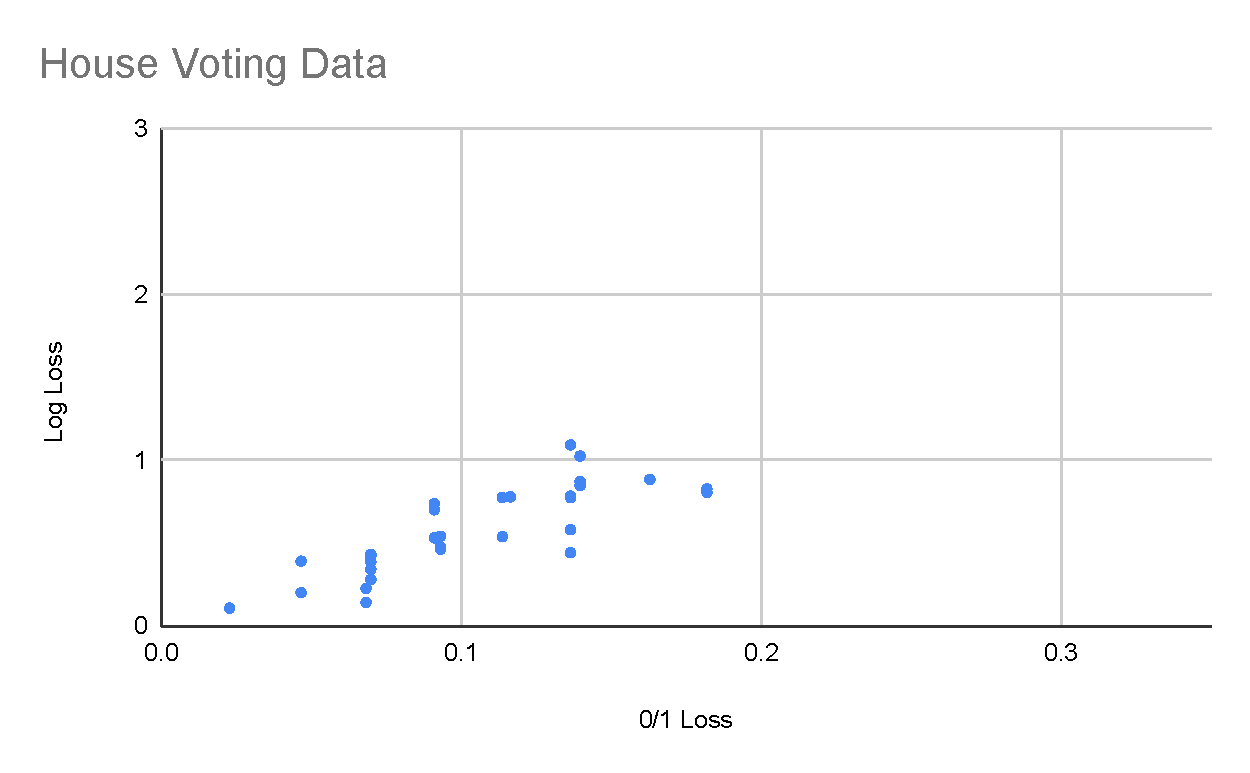
\includegraphics[width=\linewidth]{images/vote.pdf}
    \caption{Congressional Voting Data}
  \end{subfigure}
  \begin{subfigure}[b]{0.45\linewidth}
    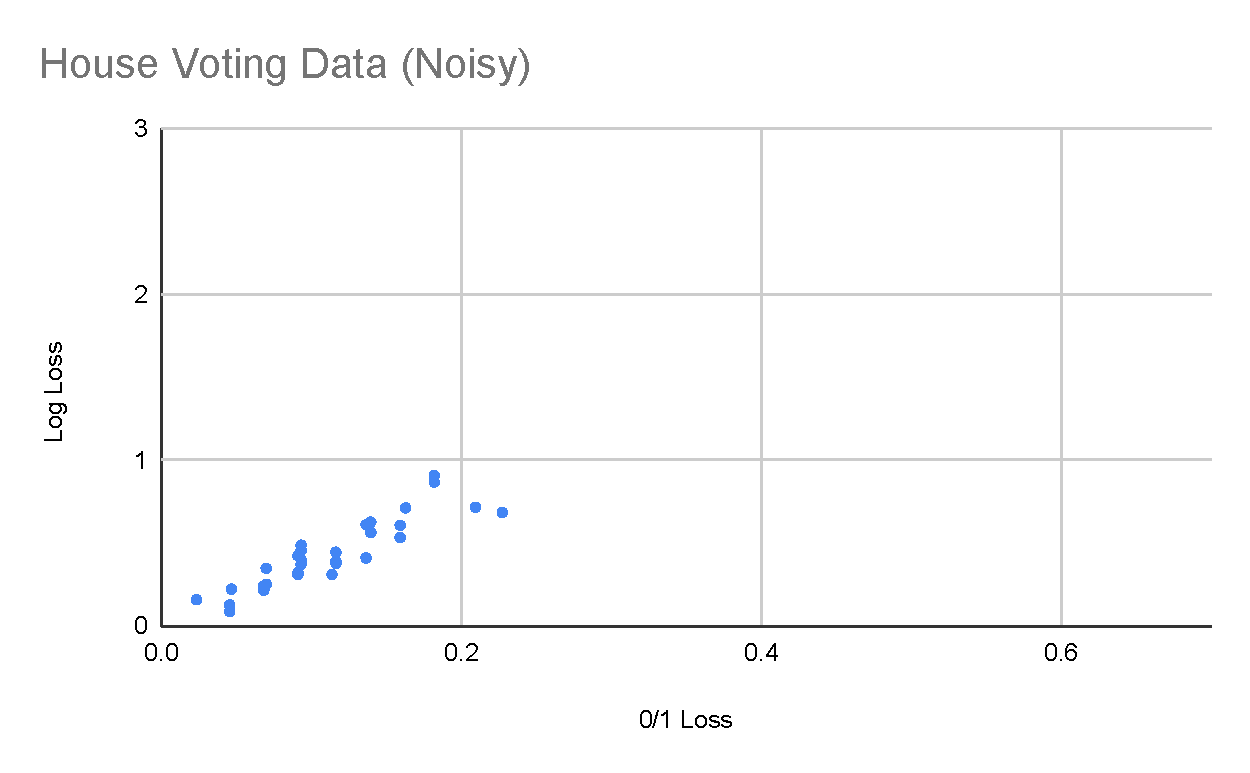
\includegraphics[width=\linewidth]{images/vote(noise).pdf}
    \caption{Perturbed Congressional Voting Data}
  \end{subfigure}
  
   \begin{subfigure}[b]{0.45\linewidth}
    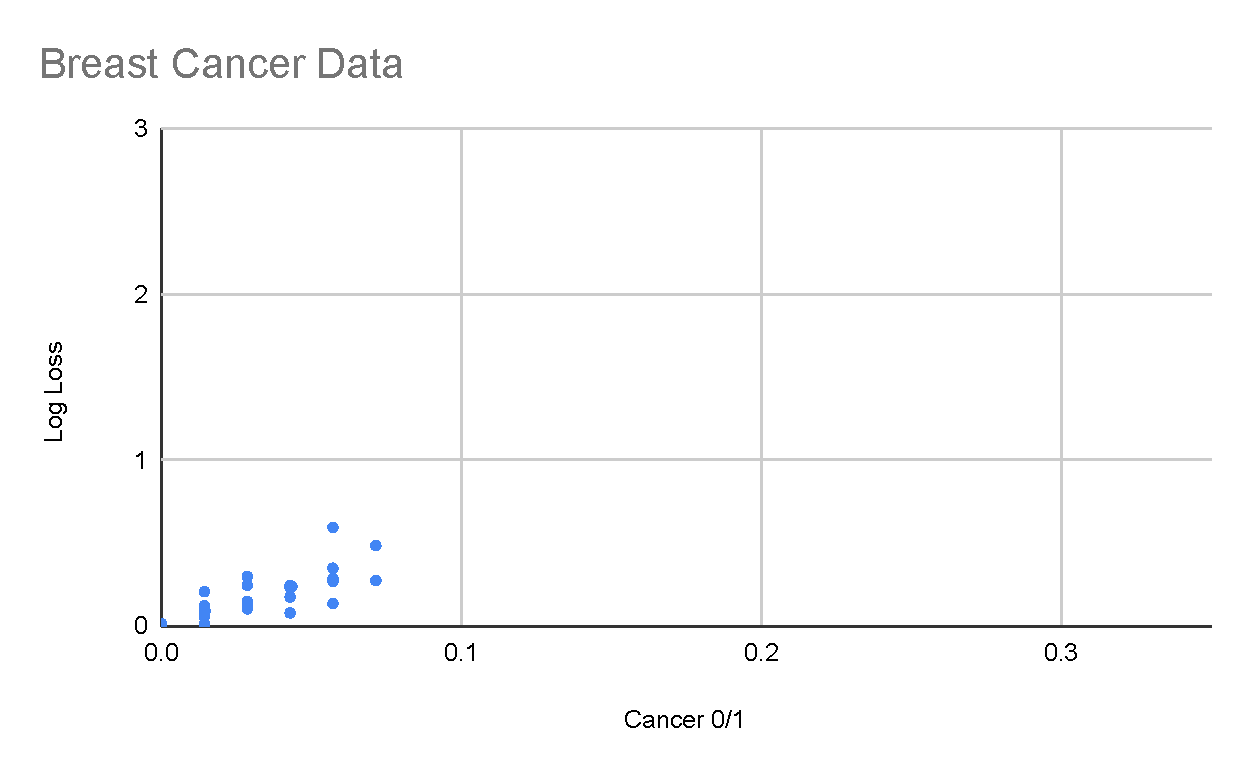
\includegraphics[width=\linewidth]{images/BC.pdf}
    \caption{Breast Cancer Data}
  \end{subfigure}
  \begin{subfigure}[b]{0.45\linewidth}
    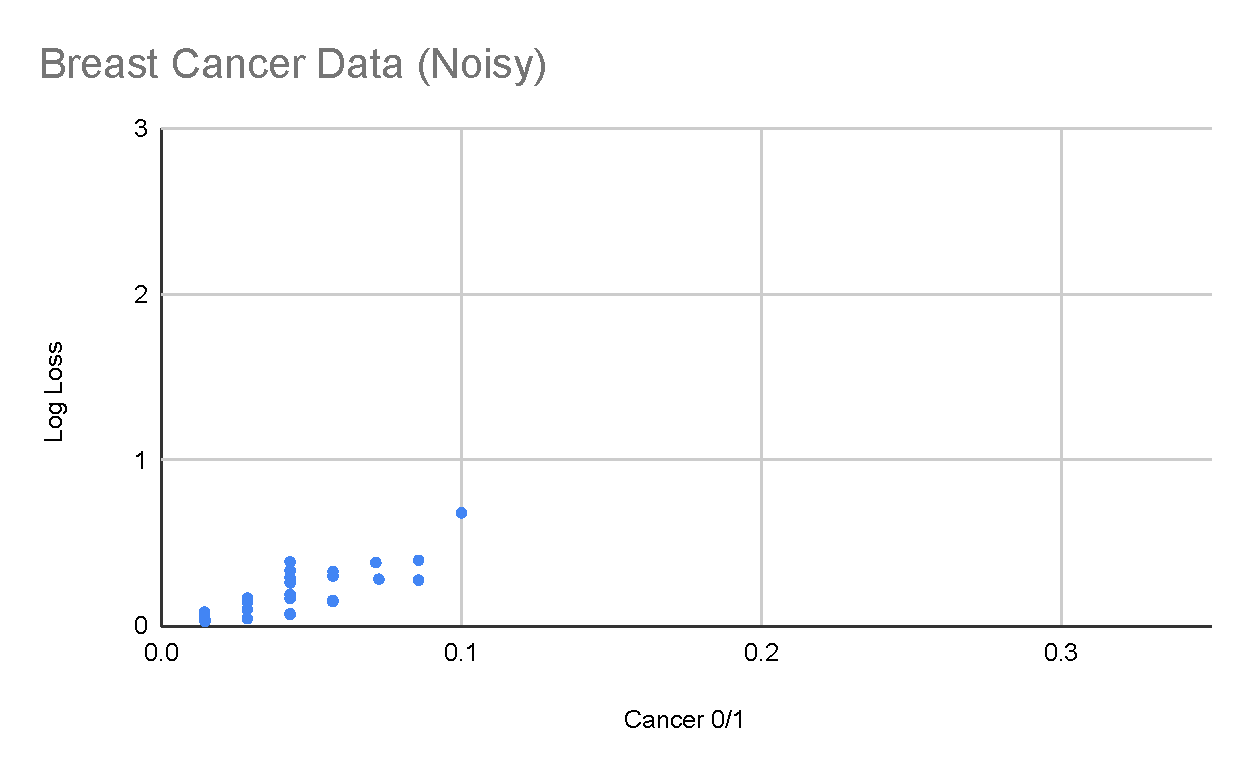
\includegraphics[width=\linewidth]{images/BC(noise).pdf}
    \caption{Perturbed Breast Cancer Data}
  \end{subfigure}
  \caption{Log Loss vs 0/1 Loss for 1984 House of Representatives Voting Data and Breast Cancer Data, which were our best performing datasets with low 0/1 and Log Loss. (Loss function evaluations are clustered in the bottom left of scatterplot)}
  \label{fig:good}
\end{figure}
  


  
\begin{figure}[h!]
 \centering
   \begin{subfigure}[b]{0.45\linewidth}
    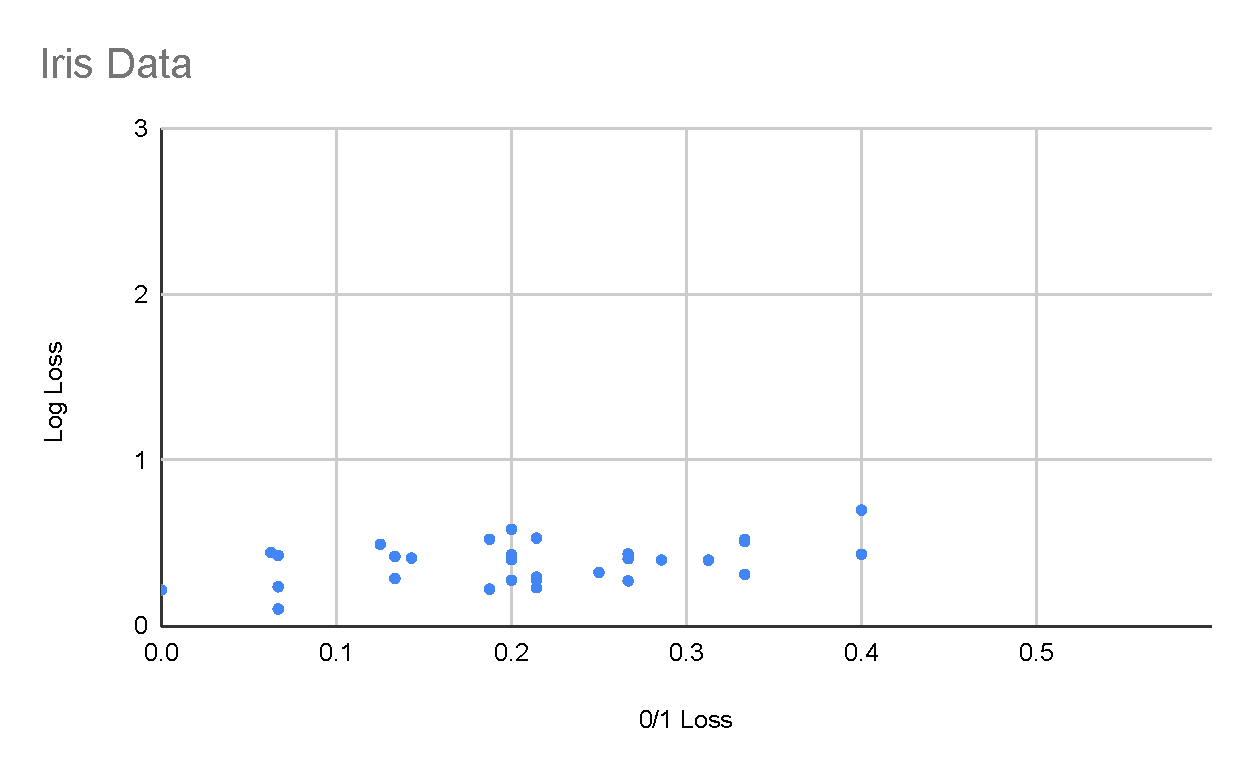
\includegraphics[width=\linewidth]{images/Iris.pdf}
    \caption{Iris Data}
  \end{subfigure}
  \begin{subfigure}[b]{0.45\linewidth}
    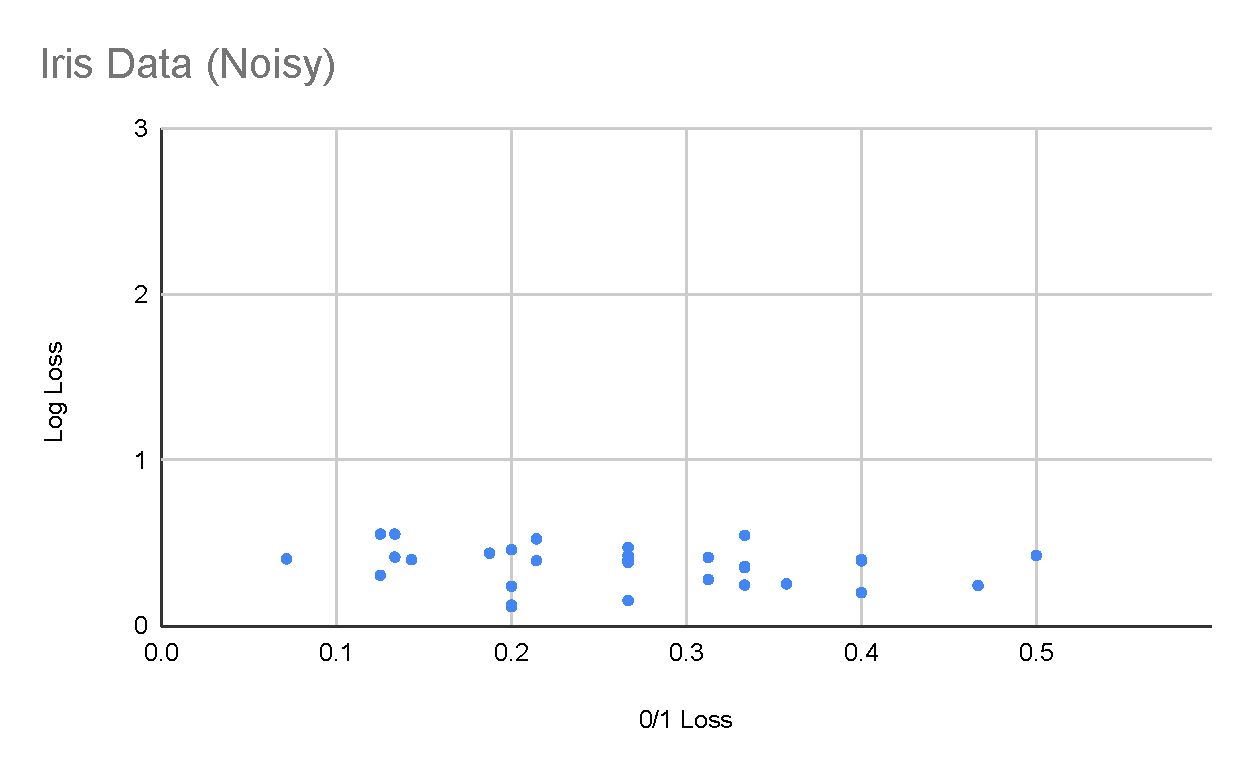
\includegraphics[width=\linewidth]{images/Iris(noise).pdf}
    \caption{Perturbed Iris Data}
  \end{subfigure}
  
  \begin{subfigure}[b]{0.45\linewidth}
     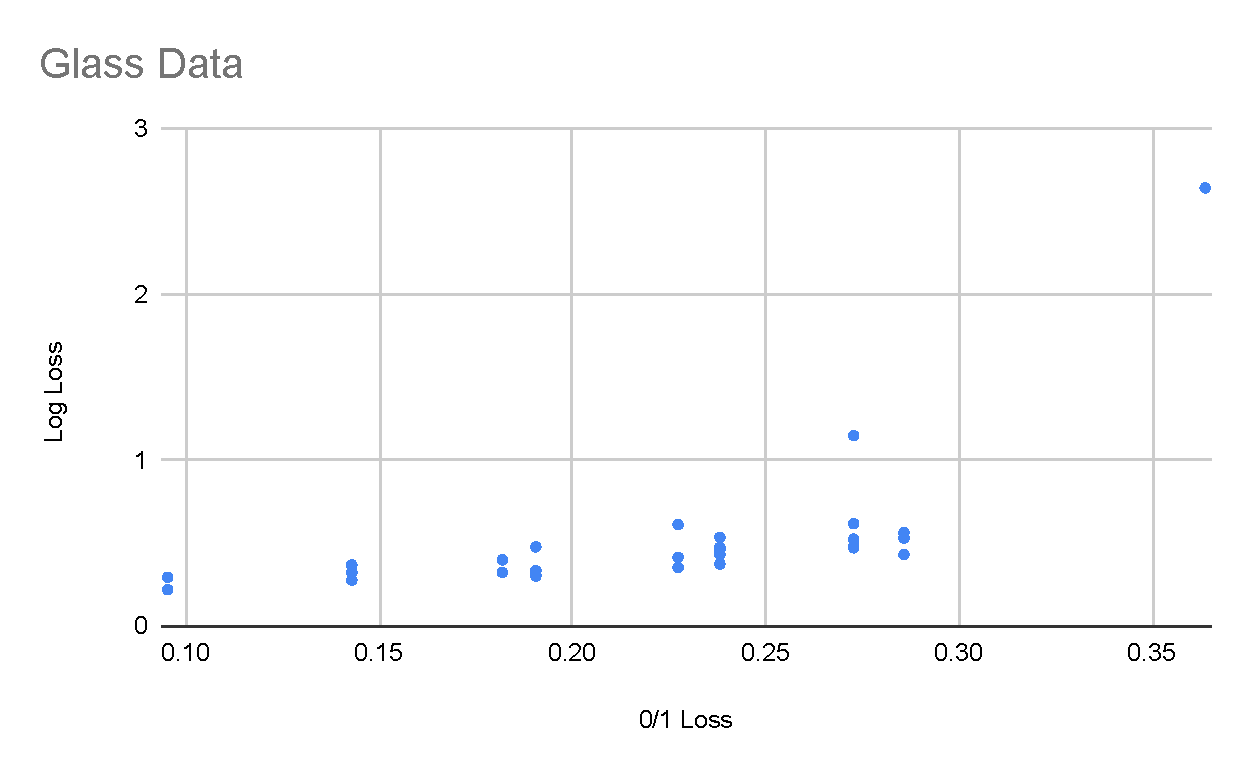
\includegraphics[width=\linewidth]{images/Gl.pdf}
    \caption{Glass Data}
  \end{subfigure}
  \begin{subfigure}[b]{0.45\linewidth}
    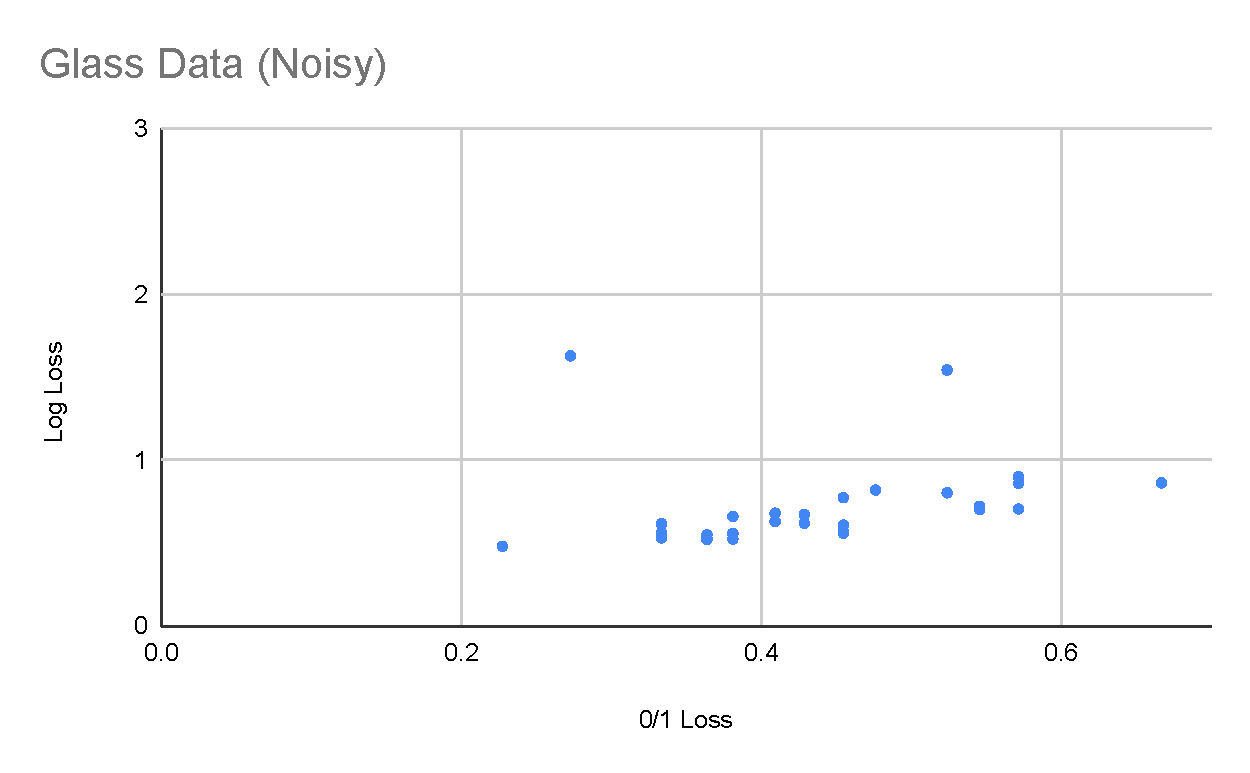
\includegraphics[width=\linewidth]{images/Gl(noise).pdf}
    \caption{Perturbed Glass Data}
  \end{subfigure}
  
   \begin{subfigure}[b]{0.45\linewidth}
    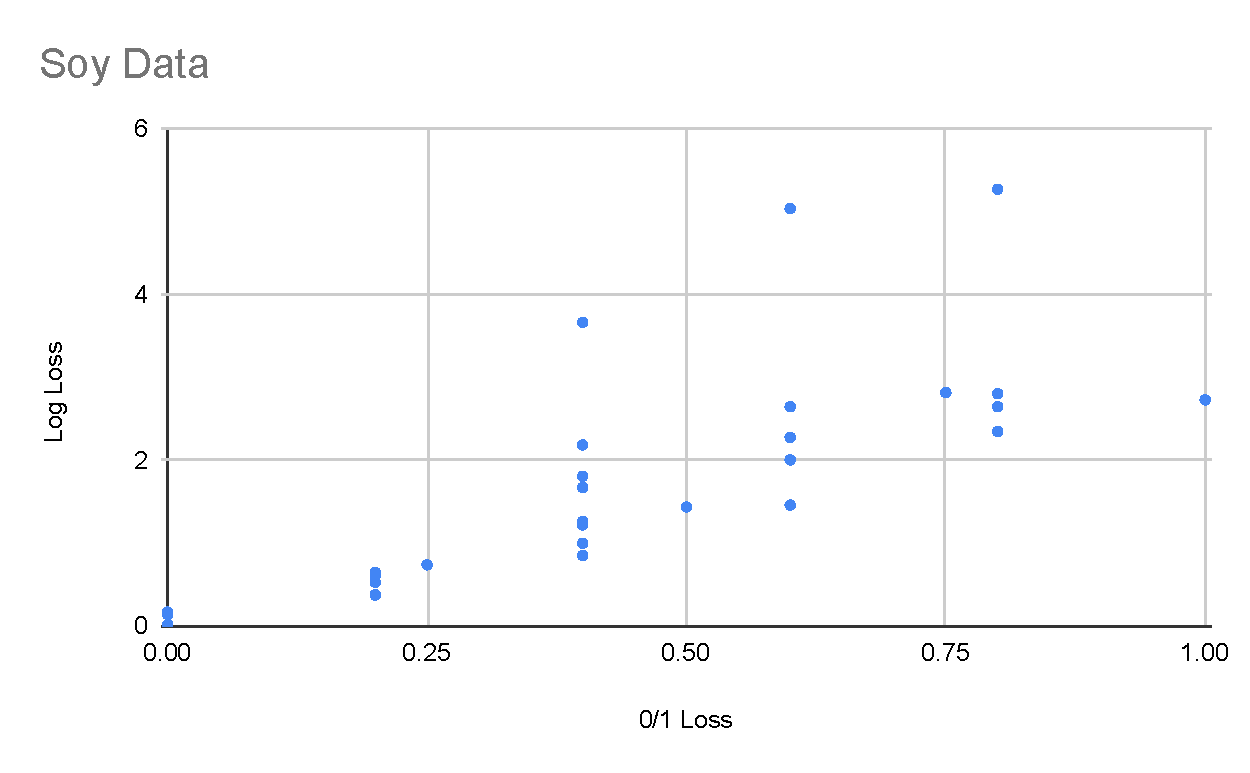
\includegraphics[width=\linewidth]{images/Soy.pdf}
    \caption{Soybean Data}
  \end{subfigure}
  \begin{subfigure}[b]{0.45\linewidth}
    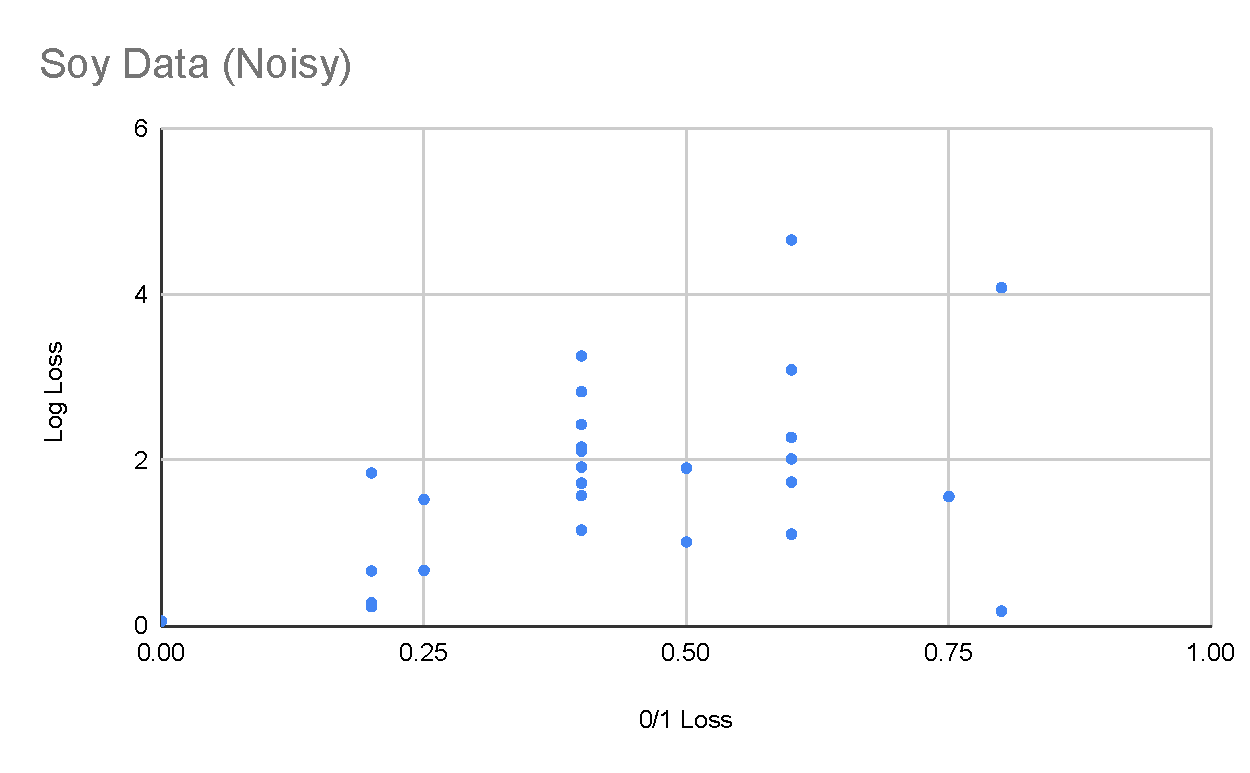
\includegraphics[width=\linewidth]{images/Soy(noise).pdf}
    \caption{Perturbed Soybean Data}
  \end{subfigure}
  
  \caption{Log Loss vs 0/1 Loss for Iris, Glass, and Soybean data. These datasets did not perform quite as well as the four datasets in \ref{fig:good}. (Loss function evaluations are more dispersed throughout the scatterplot)}
  \label{fig:ugly}
\end{figure}

\section{Discussion}
As mentioned briefly above, we found that under our model, the two best performing data sets were the 1984 house voting data and the breast cancer screening data. After this, the glass and iris
data performed similarly, hovering around the high 70\% accuracy range, with the exception of the glass data under perturbation, which performed closer to 60\% accuracy. The worst performing dataset
under both loss functions was the permuted soybean data, with an average log loss value of 1.706 and an average accuracy hovering around 56\% (meaning a 0/1 loss value of 0.4350). In contrast,
the best performing dataset by both metrics was the breast cancer data without perturbation, which achieved a log loss value of 0.1890 and a 0/1 loss value of 0.0348; implying around an average 
accuracy of 97.5\%. Perhaps for the starkest comparison, our initial hypothesis was certainly incorrect when analyzing the best and worst performing data sets. Recalling our initial hypothesis, we proposed
that more feature variables could imply better performance under a na{\"i}ve Bayes approach by a statistically significant margin- which we hypothesized to be 90\% of the time. That is, we proposed that 
a dataset with more feature variables would perform better under our two chosen loss functions than any datasets with fewer feature variables at least 90\% of the time. This certainly was not the case for our
best and worst performing datasets, as our best performing data set had only 10 feature values per line, and our worst had 35 feature values per line of data. After running the above experiment 20 times, we 
found that the breast cancer data was the best performing dataset on every run, and the soybean dataset was the worst performing dataset on every single run, directly contradicting our hypothesis. Not only 
was the largest dataset in terms of feature variables incapable of performing better than the breast cancer dataset 90\% of the time, it couldn't even do so once.
Even the smallest dataset, which contained iris data, had lower mean loss values in both metrics smaller than those of the soybean dataset on 19 in 20 runs, again directly contradicting our initial hypothesis. 
As a result, we can feel somewhat comfortable in rejecting our hypothesis that more feature values mean better performance for our model by a statistically significant margin, because in practice
the reverse was actually more often true.

These findings led us to believe that the sheer number of feature variables on any given line of data, while a factor, are not the entire picture when it comes to correctly guessing a class on some test data.
Perhaps more significant could be the number of classes in a dataset, as the two best performing datasets under our model (breast cancer and house voting datasets) were also the two with the least number of 
classes (each containing two classes). Yet, perhaps unsurprisingly, this experiment drove home that the most important aspect for a dataset to perform well under our model seems to be feature data which is 
highly correlative to its  respective class. Unearthing this kind of data might be rather tricky when considering specific, and relatively obvious aspects of a given set of data, and is certainly an ongoing area of 
work for a wide array of people throughout the machine learning community.

Despite evidence pointing us towards the rejection of our first hypothesis, our second hypothesis that our model performed worse on perturbed data than on unperturbed data was generally upheld. In 
the example run included in the table in section 3, we see that in general our hypothesis is indeed generally true, with the exception of the iris dataset under the 0/1 loss metric. It is however worth noting
that our model did perform quite well comparatively when introduced to noise, as the differences in performance were generally relatively insignificant for any dataset and its perturbed counterpart. While we 
couldn't guarantee that the average values for any given dataset would hold this trend on 90\% or more repetitions of our experiment, it was certainly true for multiple datasets and was nearly true for others.
Relaxing the percentage from 90\% might present an interesting avenue of future work as well, as it was nearly the case that our model performed better on every dataset without perturbations at least 90\% of
the time.




\section{Summary}
Within this project, we describe our findings while running a Naive Bayesian algorithm on a multitude of datasets. On each dataset, we ran a version with and without noise to evaluate how our model handles variations in the data. Using two different loss functions, we are able to obtain a quantifiable measure of performance on each model. Our hypotheses were that our model would perform better on data with a higher quantity of attributes and on datasets with less noise introduced. After running multiple ten-fold cross validation tests, we discovered that the model generally performed worse on datasets with more attributes, proving our original hypothesis incorrect. However, the model performed consistently better on the non-permuted data, which is in line with our hypothesis. Throughout this project, we identified many avenues of improvement for future models. In the future, it would be interesting to explore further cross validation to determine optimal hyperparameters. Additionally, we would explore additional loss functions to see how they differ in measuring model performance. Overall, this project offered an effective introduction into the field of machine learning and an exciting opportunity to perform a range of experiments and implement a classic learning algorithm

\vskip 0.2in

\end{document}
